%\def\DEBUG{1}
\ifdefined\DEBUG
\documentclass[11pt,twoside]{mitthesis}
\usepackage{tikz}
\usepackage{circuitikz}
\usepackage{amsmath}
\usepackage{fancyvrb}
\usepackage{float}
\newcommand{\ohm}{$\Omega$ }
\begin{document}
\fi

\chapter{Results}
In this chapter, results for the simulation and hardware implementations of the RLC network identifying system are presented and analyzed.
The shortcomings of the systems are addressed and potential improvements are discussed as future work.

\section{Simulation Performance}
The performance of the RLC network identification system simulator is analyzed by its output precision and cases in which it fails.
The output precision of the simulator is quite good and can be controlled almost arbitrarily.
The precision depends almost entirely on the thresholds defined during the finite-differencing step, as looser thresholds allow bad data to get averaged into the good data.
The cases in which the simulator fails are always cases where a relatively high resistance is in parallel with an LC network.
In these cases, the simulator reports that there is no resistor in parallel with the LC network.
The failure mode lies within finite difference stencil thresholding, where the simulator never finds a region where the slope of the impedance vs frequency plot is zero, and in turn the simulator decides there is no resistor.
Designing a better element identifying algorithm would make excellent future work.

The schematic renderer used to display the returned matrices as a legible schematic could use some work as well.
It is effective at creating schematics for circuits composed of resistors with only a few nodes, but the value labeling system and lack of organization quickly gets out of hands when the number of nodes is greater than five.
There has been a fair bit of research into auto-generating schematics from netlists, particularly from the days of discrete digital logic, such as \emph{ASG [Automatic Schematic Generator]} from Lageweg at Delft University \cite{delft} and the \emph{ASG} from Jehng, Chen, and Parng at National Taiwan University \cite{taiwan}.


%This could be remedied by either a patch to the algorithm or another algorithm entirely.
%Instead of using a slope of zero on the \texttt{|Z| vs. f} plot to indicate parallel resistance, the maximum recorded impedance can be taken as the parallel resistance whenever the simulator finds an LC circuit.
%In the case of an LC circuit where there is no resistance, 

\section{Hardware Performance}

The hardware RLC network identification system was tested to determine its dynamic range of operation, precision, and ability to detect RLC networks.

\subsection{Element Testing}
\subsubsection{Resistance}
A selection of resistors ranging from 33\ohm to 330k\ohm were analyzed with the RLC network identification system.  
For each resistor, the identified resistance was recorded and plotted. 

\begin{figure}[H]
	\label{fig:rplot}
  \begin{center}
      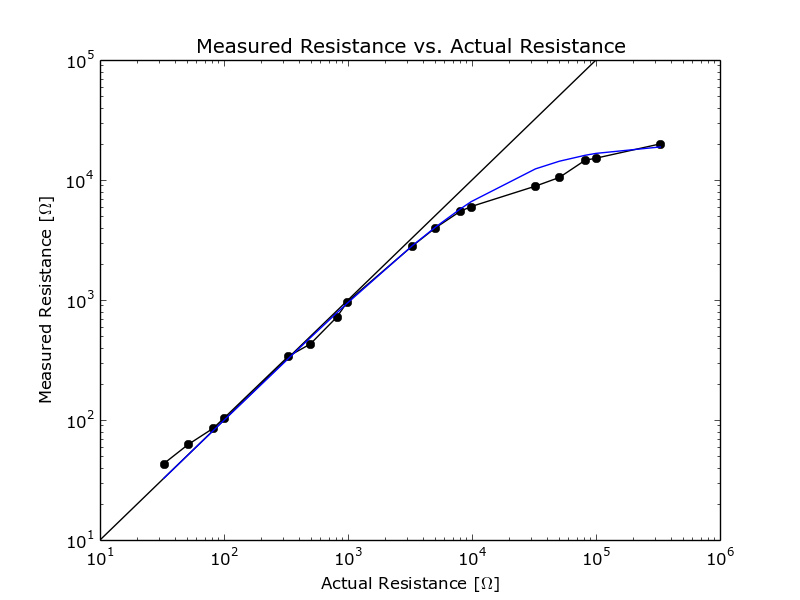
\includegraphics[width=.7\textwidth]{../rin-ro.png}
      \caption{Plot of measured resistance for known resistors}
  \end{center}
\end{figure}

From the Figure \ref{fig:rplot}, the range of resistances for which the system maintains valid precision operation is between $\sim100$ and 2000\ohm.
For resistances larger than 2k\ohm, the system returns resistances that are far smaller than the input resistance.
The asymptotic portion of the curve in Figure \ref{fig:rplot} indicates a parallel resistance somewhere around 20k\ohm.
The blue line indicates the equivalent resistance of each tested resistance with a parallel 20k\ohm resistor.
This parallel resistance is not real.
Using an ohmmeter, it was verified that there is not enough leakage current between breadboard nodes or between breadboard nodes and ground to account for 20k\ohm of resistance.
Rather, this measurement error is caused by the minimum non-zero signal amplitude measured on the output of the current amplifier A/D converter.
A 10-bit ADC that samples a $5V$ window converts every $.004V$ into one bit.
The minimum amplitude signal produced by a 10-bit ADC sampling over a $5V$ scale has an amplitude of $4mV$.
The test voltages applied to each node have amplitudes around $0.75V$.
The current amplifier has a gain of 100, so the effective current amplitude measured is $40\mu A$. 
\quad \qquad \qquad \qquad \qquad \qquad $0.75V / 40\mu A=18750\Omega$\\
So, the maximum possible impedance measurement from any node to ground, $R_{n_{||}}$, is 19k\ohm.
A frequency sweep of the impedance of an open node, such as the one in Figure \ref{fig:zopen}, demonstrates this.
\begin{figure}[H]
	\label{fig:zopen}
  \begin{center}
      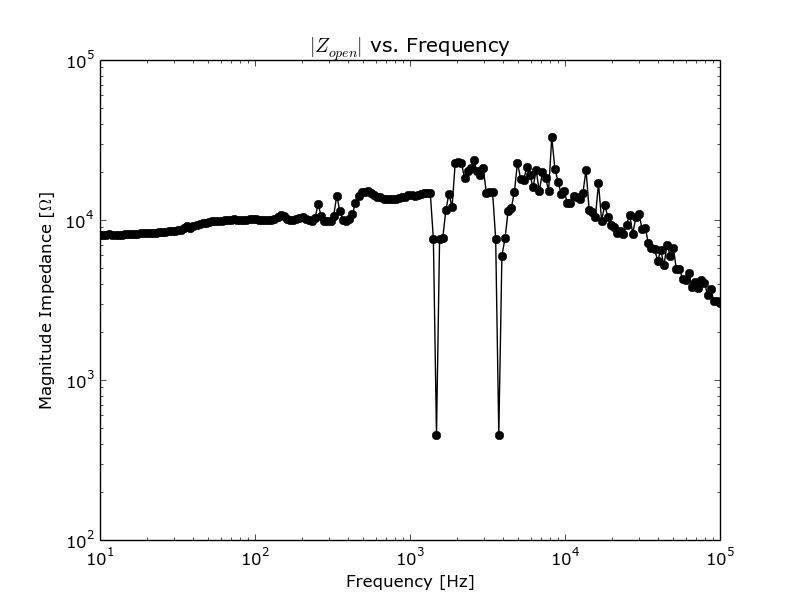
\includegraphics[width=.7\textwidth]{../zopen-gnd.png}
      \caption{Driving point impedance of an open node from 1Hz to 100KHz}
  \end{center}
\end{figure}
By adding a variable gain stage to the current amplifier, or a variable-sized sense resistor, the maximum impedance measurement could be modified.

The maximum impedance measurement between two nodes, rather than just one node to ground, is an order of magnitude higher.
This is due to the procedure used in the network sensing algorithm, where $V_t R_{n_{||}}$ is divided by $V_m$.
If $V_n$ is smaller than 1, the resulting resistance $R_{nm}$ is larger than $R_{n_{||}}$

\begin{figure}[h]
	\label{fig:z2open}
  \begin{center}
      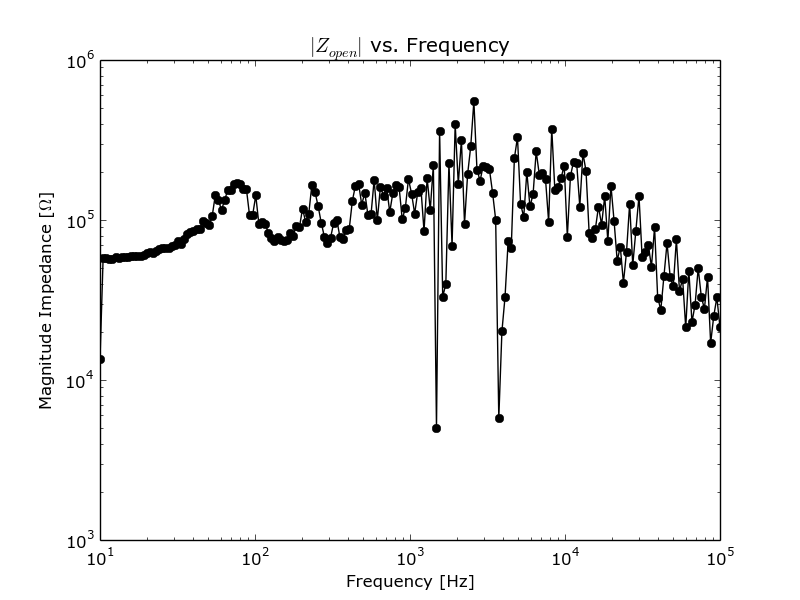
\includegraphics[width=.7\textwidth]{../zopen.png}
      \caption{Impedance between two open nodes from 1Hz to 100KHz}
  \end{center}
\end{figure}

On the other side of Figure \ref{fig:rplot}, for resistances smaller than 100\ohm the system returns resistances that are far larger than the input resistance.
This can be attributed to the DAC buffer current limit, which is $\pm25mA$.
For a test voltage signal of $\sim1.5V$, a 60\ohm resistance produces a $25mA$ current.
This agrees with the recorded data quite well.
To measure resistances smaller than 100\ohm the output buffer could be replaced with one that has a higher output current limit.
Alternatively, a variable-sized sense resistor would also mitigate the problem.

\subsubsection{Capacitance}

In addition to the resistors, a selection of capacitors ranging from $220pF$ to $22\mu F$ were analyzed with the RLC network identification system.  
For each capacitor, the identified capacitance was recorded and plotted in Figure \ref{fig:cplot}.

\begin{figure}[h]
	\label{fig:cplot}
  \begin{center}
      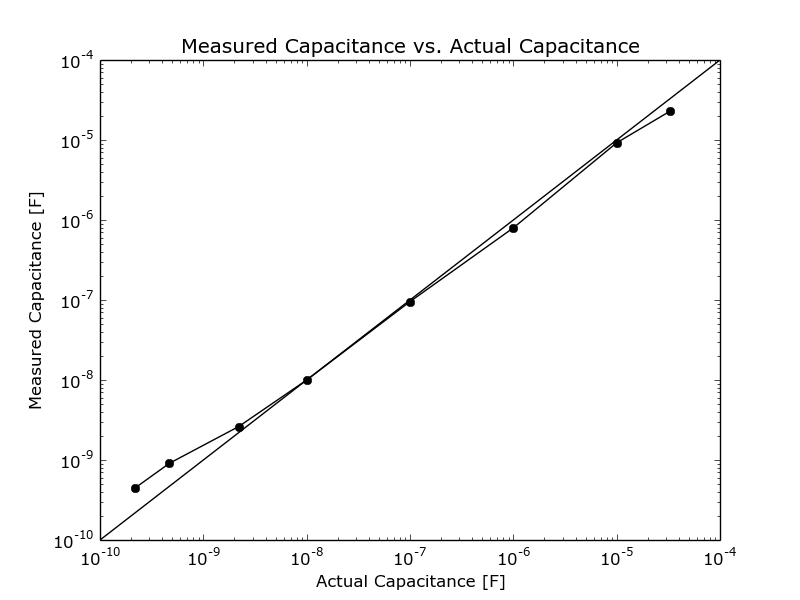
\includegraphics[width=.7\textwidth]{../cin-co.png}
      \caption{Plot of measured capacitance for known capacitors}
  \end{center}
\end{figure}

The RLC network identification system can precisely measure capacitances over three orders of magnitude, from $2.2nF$ to $10\mu F$.
On the low end of Figure \ref{fig:cplot}, the parallel parasitic capacitance is visible, which adds about $150pF$ to the system, although this does not entirely account for the measured capacitance.
On the high end, the impedance of the capacitors at the test frequencies drops below 50\ohm, again causing the buffer op-amp to reach its output current limits and saturate.
The working range of $1nF$ to $10\mu F$ is acceptable for general purposes.

\subsubsection{Inductance}



A selection of inductors ere analyzed with the RLC network identification system to no avail.
The identification system was not able to find the inductors due to the noisy nature of the impedance measurements that inductors were found to return.


The 'noisy' impedance, shown in Figure \ref{fig:lplot}, defeats the finite-differencing technique, and causes it to return a large (amplitude of 20) random-looking signal.
This is much larger than the +1 output that is expected for an inductor, and causes the element identification step to fail.

In addition to recording noisy measurements while attempting to identify an inductor alone, noisy measurements were found when attempting to identify RL, LC, and RLC parallel circuits.
One would expect to find noisy inductive data in the section of the plot where the inductor dominates and and clean capacitive or resistive data in the sections of the plot where the capacitor or resistor dominates, but this is not the case.
This issue has not been closed, yet is integral to the acceptable operation of an RLC network identification system.
Identifying and solving this problem would make excellent future work.

\begin{figure}[h]
	\label{fig:lplot}
  \begin{center}
      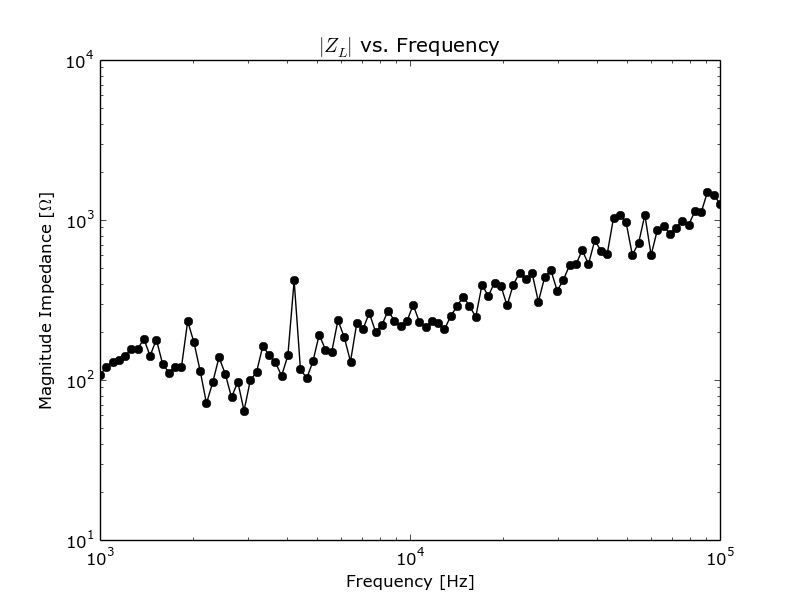
\includegraphics[width=.7\textwidth]{../zl.png}
      \caption{Impedance vs frequency for a $3.3mH$ inductor, demonstrating inductive behavior albeit noisily}
  \end{center}
\end{figure}

\begin{figure}[H]
	\label{fig:lcplot}
  \begin{center}
      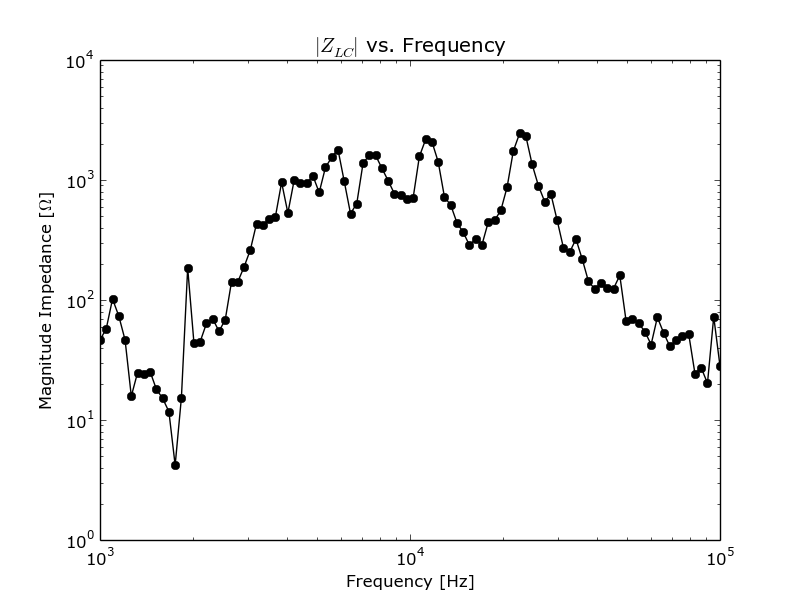
\includegraphics[width=.7\textwidth]{../zlc.png}
      \caption{Impedance vs frequency for a $3.3mH$ inductor in parallel with a $0.15\mu F$ capacitor, demonstrating LC behavior albeit noisily}
  \end{center}
\end{figure}
\newpage
\subsection{Network Testing}

To verify the network identification system performed properly, complete networks of three, four, five, and six nodes were constructed from resistors within the range of 100\ohm to 1000\ohm.

\begin{figure}[H]
	\label{fig:nodes}
		\begin{center}
      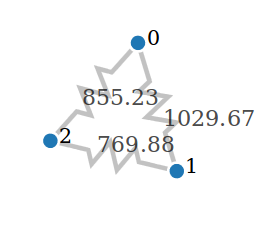
\includegraphics[width=.4\textwidth]{../3node.png}
      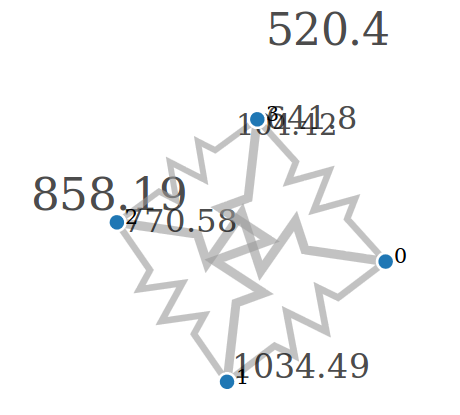
\includegraphics[width=.4\textwidth]{../4node.png}
      \end{center}
      \begin{center}
      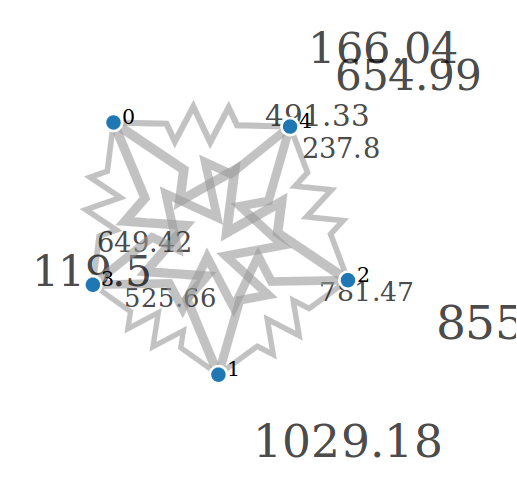
\includegraphics[width=.4\textwidth]{../5node.png}
      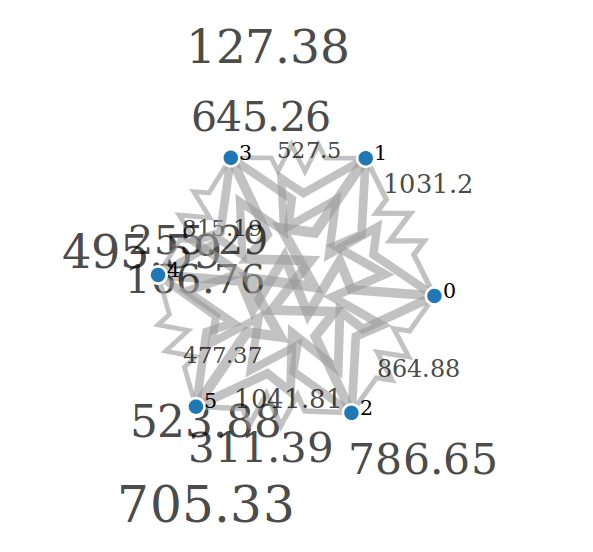
\includegraphics[width=.4\textwidth]{../6node.png}
      \end{center}
      \caption{Schematics of 3, 4, 5, and 6-node resistor networks rendered in the browser}
\end{figure}
  
\begin{Verbatim}[fontsize=\footnotesize]
R
None     1.03e+03 8.55e+02  
1.03e+03 None     7.70e+02  
8.56e+02 7.71e+02 None  
\end{Verbatim}


\begin{Verbatim}[fontsize=\footnotesize]
R

None     1.03e+03 8.58e+02 6.42e+02  
1.03e+03 None     7.71e+02 5.20e+02  
8.63e+02 7.84e+02 None     1.04e+02  
6.46e+02 5.27e+02 1.04e+02 None      
\end{Verbatim}

\begin{Verbatim}[fontsize=\footnotesize]
R

None     1.03e+03 8.56e+02 6.49e+02 4.91e+02  
1.04e+03 None     7.81e+02 5.26e+02 1.66e+02  
9.99e+02 8.87e+02 None     1.19e+02 2.38e+02  
6.66e+02 5.31e+02 1.05e+02 None     6.55e+02  
5.02e+02 1.67e+02 2.10e+02 6.54e+02 None 
\end{Verbatim}

\begin{Verbatim}[fontsize=\footnotesize]
R

None     1.03e+03 8.65e+02 6.45e+02 4.96e+02 5.24e+02  
1.04e+03 None     7.87e+02 5.28e+02 1.67e+02 7.05e+02  
1.06e+03 9.65e+02 None     1.27e+02 2.55e+02 1.04e+03  
8.10e+02 6.60e+02 1.31e+02 None     8.15e+02 3.11e+02  
5.57e+02 1.91e+02 2.39e+02 7.67e+02 None     4.77e+02  
5.19e+02 6.97e+02 8.51e+02 2.49e+02 4.12e+02 None     
\end{Verbatim}

\section{Improvements}
\subsection{VGA for ADC's, DAC, and Differential Amplifier}
\subsection{Variable Sense Resistor}
\subsection{Better Switches}
\subsection{Computer-Aided Debugger}
\subsection{Three Terminal Devices}
\subsection{Better Schematic Display}

\section{Conclusion}
\ifdefined\DEBUG
\end{document}
\fi